\documentclass{article}

%% MasteryNotebookTemplate.tex (c) by Emma Smith Zbarsky
%% MasteryNotebookTemplate.tex is licensed under a
%% Creative Commons Attribution 3.0 Unported License.

%%You should have received a copy of the license along with this
%%work.  If not, see <http://creativecommons.org/licenses/by/3.0/>.

\usepackage[usenames,dvipsnames]{color}
\usepackage{amssymb,amsmath, multirow}
\usepackage[initials]{amsrefs}
\usepackage{fullpage}
%\usepackage[all]{xy}
\usepackage{mathrsfs} %% for \mathscr and \mathfrak
\usepackage{graphicx} %% for \includegraphics

%% New stuff
\usepackage[pdftex,plainpages=false,hypertexnames=false,pdfpagelabels]{hyperref}
\usepackage{xcolor}
\definecolor{dark-red}{rgb}{0.7,0.25,0.25}
\definecolor{dark-blue}{rgb}{0.15,0.15,0.55}
\definecolor{medium-blue}{rgb}{0,0,0.65}
\hypersetup{
  colorlinks, linkcolor={purple},
  citecolor={medium-blue}, urlcolor={medium-blue}
}
%% End New Stuff

%\theoremstyle{hharemark}
\newtheorem{theorem}{Theorem}[section]
\newtheorem{proposition}[theorem]{Proposition}
\newtheorem{lemma}[theorem]{Lemma}
\newtheorem{corollary}[theorem]{Corollary}
\newtheorem{definition}[theorem]{Definition}
\newtheorem{assumption}[theorem]{Assumption}
\newtheorem{remark}{Remark}

\def\R{\mathbb{R}}
\def\Z{\mathbb{Z}}
\def\ds{\displaystyle}
\def\der#1#2{\frac{\partial #1}{\partial #2}} % partial derivatives
\def\d#1#2{\frac{d#1}{d#2}} % standard derivatives
\def\dt#1#2{\frac{d^2#1}{d#2^2}}
\def\dth#1#2{\frac{d^3#1}{d#2^3}}
\def\com#1{\texttt{#1}}
\def\x{\mathbf{x}}
\def\v{\mathbf{v}}
\def\bpm{\begin{pmatrix}}
\def\epm{\end{pmatrix}}
\def\O{\mathcal{O}}
\newcommand{\checked}{\makebox[0pt][l]{$\checkmark$}$\square$}
\newcommand{\unchecked}{$\Box$}
%\Theoremstyle{remark}

% Bernard Deconinck's macros
\newcommand{\beq}{\begin{equation}}
\newcommand{\eeq}{\end{equation}}
\newcommand{\ba}{\begin{array}}
\newcommand{\ea}{\end{array}}
\newcommand{\bea}{\begin{eqnarray*}}
\newcommand{\eea}{\end{eqnarray*}}
\newcommand{\bc}{\begin{center}}
\newcommand{\ec}{\end{center}}
\newcommand{\bt}{\begin{table}}
\newcommand{\et}{\end{table}}
\newcommand{\la}[1]{\label{#1}}
\newcommand{\p}{\partial}
\newcommand{\pp}[2]{{\partial #1 \over \partial #2}}
\newcommand{\ppn}[3]{{\partial^{#1} #2 \over \partial #3^{#1}}}
\newcommand{\mbf}[1]{\mbox{\boldmath {$#1$}}}
\newcommand{\red}[1]{\textcolor{red}{#1}}
\newcommand{\green}[1]{\textcolor{green}{#1}}
\newcommand{\blue}[1]{\textcolor{blue}{#1}}
\newcommand{\yellow}[1]{\textcolor{yellow}{#1}}
\newcommand{\purple}[1]{\textcolor{purple}{#1}}
\newcommand{\black}[1]{\textcolor{black}{#1}}
%\definecolor{RawSienna}{rgb}{.4,.2,0}
\begin{document}
\begin{titlepage}
  \begin{center}
    \bfseries
\huge Mastered Learning Objectives \\  from \\ Partial Differential Equations \\[.5in]
\large MATH 4900, Fall 2020 with Prof. Emma Zbarsky
\vfill
\includegraphics[height=3.5in, angle=90]{coolimage}
\vfill
\LARGE James Slowik \\[.2in]
\texttt{slowikj@wit.edu}
%\address{550 Huntington Ave,
%               Boston, MA 02115
%         USA}
%\thanks{You could thank grant support here.}
\end{center}      
\end{titlepage}
\newpage
\tableofcontents
\newpage
% Text of Document.  Use constructs such as \section, \subsection,
% \begin{theorem} ... \end{theorem}, \begin{proof} ... \end{proof}, etc.
\section{Mastery Check Planning}
% To check a box in the Productive Failure? column, replace the code \unchecked with \checked and recompile. 
\begin{tabular}{|l|c|c|c|c} \cline{1-4}
\multirow{2}{5cm}{\textbf{Standard}} & Suggested & Mastery Date & Writeup & Productive  \\ 
& Date & & Completed & Failure? \\ \cline{1-4}
\multirow{2}{5cm}{NM: Order of Error} & \multirow{2}{1.5cm}{Wk 2} & 9/18/20 & 9/26/20 & \multirow{2}{.4cm}{\unchecked} \\ &&&& \\ \cline{1-4}
\multirow{2}{5cm}{NM: Explicit Difference} & \multirow{2}{1.5cm}{Wk 3} &     &           & \multirow{2}{.4cm}{\unchecked} \\ &&&& \\ \cline{1-4}
\multirow{2}{5cm}{MC: Linear, constant speed}  & \multirow{2}{1.5cm}{Wk 3} & 10/2/20 & 11/29/20 & \multirow{2}{.4cm}{\checked} \\ &&&& \\ \cline{1-4}
\multirow{2}{5cm}{MC: Linear, polynomial speed} & \multirow{2}{1.5cm}{Wk 4} & 10/2/20 & 11/30/20 & \multirow{2}{.4cm}{\unchecked} \\ &&&& \\ \cline{1-4}
\multirow{2}{5cm}{MC: Nonlinear} &\multirow{2}{1.5cm}{Wk 4}&&& \multirow{2}{.4cm}{\unchecked} \\ &&&& \\ \cline{1-4}
\multirow{2}{5cm}{MC: Shock} &\multirow{2}{1.5cm}{Wk 5}&      &           & \multirow{2}{.4cm}{\checked} \\ &&&& \\ \cline{1-4}
\multirow{2}{5cm}{MC: Rarefaction} & \multirow{2}{1.5cm}{Wk 5}&      &         &  \multirow{2}{.4cm}{\unchecked} \\ &&&& \\ \cline{1-4}
\multirow{2}{5cm}{NM: Neumann stability} &\multirow{2}{1.5cm}{Wk 6}&&& \multirow{2}{.4cm}{\unchecked} \\ &&&& \\ \cline{1-4}
\multirow{2}{5cm}{NM: CFL condition} &\multirow{2}{1.5cm}{Wk 6} & 10/22/20 & 12/9/20 &  \multirow{2}{.4cm}{\unchecked} \\ &&&& \\ \cline{1-4}
\multirow{2}{5cm}{NM: Implicit Difference} &\multirow{2}{1.5cm}{Wk 6}&&& \multirow{2}{.4cm}{\unchecked} \\ &&&& \\ \cline{1-4}
\multirow{2}{5cm}{FS: Real Fourier Series} & \multirow{2}{1.5cm}{Wk 7}  & 10/29/20 & 12/1/20 &  \multirow{2}{.4cm}{\unchecked} \\ &&&& \\ \cline{1-4}
\multirow{2}{5cm}{FS: Complex Fourier Series} & \multirow{2}{1.5cm}{Wk 7} & 11/6/20 & 12/1/20 & \multirow{2}{.4cm}{\unchecked} \\ &&&& \\ \cline{1-4}
\multirow{2}{7cm}{FS: Convergence of Fourier Series} & \multirow{2}{1.5cm}{Wk 8} &&& \multirow{2}{.4cm}{\unchecked} \\ &&&& \\  \cline{1-4}
\multirow{2}{7cm}{FS: Integrability \& Differentiability of FS} & \multirow{2}{1.5cm}{Wk 8} & 11/13/20 &         & \multirow{2}{.4cm}{\unchecked} \\ &&&& \\  \cline{1-4}
\multirow{2}{5cm}{FS: Boundary Conditions} & \multirow{2}{1.5cm}{Wk 9} &&& \multirow{2}{.4cm}{\unchecked} \\ &&&& \\ \cline{1-4}
\multirow{2}{5cm}{SV: Heat Equation} & \multirow{2}{1.5cm}{Wk 10} & 11/19/20 & 12/3/20 & \multirow{2}{.4cm}{\unchecked} \\ &&&& \\ \cline{1-4}
\multirow{2}{5cm}{SV: Equilibrium behavior} & \multirow{2}{1.5cm}{Wk 10} & 11/20/20 & 12/3/20 & \multirow{2}{.4cm}{\unchecked} \\ &&&& \\ \cline{1-4}
\multirow{2}{5cm}{SV: Wave equation} & \multirow{2}{1.5cm}{Wk 11} &      &            & \multirow{2}{.4cm}{\checked} \\ &&&& \\ \cline{1-4}
\multirow{2}{5cm}{SV: d'Alembert's equation} & \multirow{2}{1.5cm}{Wk 12} &&& \multirow{2}{.4cm}{\unchecked} \\ &&&& \\ \cline{1-4}
\multirow{2}{5cm}{SV: Laplace equation} & \multirow{2}{1.5cm}{Wk 13} &&& \multirow{2}{.4cm}{\unchecked} \\ &&&& \\ \cline{1-4}
\multirow{2}{5cm}{Final Preparations} & \multirow{2}{1.8cm}{Wk 14/15} &&&   \\&&&& \\ \cline{1-4}
\end{tabular}
\newpage
%\section{Numerical Methods}
\section{Numerical Methods of Solving Partial Differential Equations}
%\red{Give a brief overview of this section of the class. The following would be a sample introduction to such a section from an ordinary differential equations class.}

Numerical Methods aim to solve PDE's by successively iterating a numerical scheme to generate points in a mesh that represent the solution to a PDE. Each point in the mesh represents the specific solution for a certain point in space and time. The numerical methods we use are formed from approximations of the derivatives in the PDE, like Euler's forward, backward, and centered difference formulas. We can plug in these approximations of the derivatives to solve for the equation that gives the value at the next time step and same point in space. Additionally, we need to choose a value for $\Delta t$ and $\Delta x$ - how much the method moves forward in space and time for each iteration. These are usually small, since we want an accurate approximation of the solution. 
% Don't forget to delete all of the commentary and sample code before you submit this as your Mastery Notebook.

%A first order initial value problem takes the form \(\ds \d{y}{t} = f(y,t)\) with \(\ds y(t_0)=y_0\). Such functions are studied in a first class on differential equations in a variety of special cases (e.g. separable equations or linearequations) but there is no general analytic method that works for every \(f\). We shall explore some numerical methods of finding a solution.

\subsection{Order of Error}
%\blue{Explain how you calculate the order of the error in a finite difference approximation scheme here. You should illustrate your explanation by solving at least the problem I gave you to demonstrate mastery. If you wish to include others as well that is up to you. What follows is a sample bit of text discussing the order of the error for the Euler Method of solving ODEs.} \newline

The Order of Error in a finite difference approximation tells us how fast the error term, that comes from approximating a function, changes when we increase or decease the step size.\newline

The mastery problem I was given: Approximate $u'(x)$ with $u(x)$, $u(x-3h)$, and $u(x-2h)$. What is the optimal order of error? \newline

To calculate the order of the error, we first use a Taylor Series to expand each function used to approximate the derivative except $u(x)$

\bea
u(x-3h) &=& u(x) - u'(x)(3h) + \dfrac{u''(x)(3h)^2}{2!} -  \dfrac{u'''(x)(3h)^3}{3!}+\ldots \\
u(x-2h) &=& u(x) - u'(x)(2h) + \dfrac{u''(x)(2h)^2}{2!} - \dfrac{u'''(x)(2h)^3}{3!}+\ldots
\eea

We want to solve for $u'(x)$ so lets begin by putting coefficients in front of each term in the expansions. This will allow us to combine the expansions and helps us cancel higher order terms. You need as many coefficients as you have expansions. We have 2 so we need A and B.\newline
We now have: \newline
\bea
Au(x-3h) &=& Au(x) - Au'(x)(3h) + A\dfrac{u''(x)(3h)^2}{2!} -  A\dfrac{u'''(x)(3h)^3}{3!}+\ldots \\
Bu(x-2h) &=& Bu(x) - Bu'(x)(2h) + B\dfrac{u''(x)(2h)^2}{2!} - B\dfrac{u'''(x)(2h)^3}{3!}+\ldots
\eea

Solve for A and B. We want the coefficients of each term in their expansions to add to 0. Don't include the term were solving for. In this case, don't include $u'(x)$. \newline
\bea
u(x): A + B = 0 \\
u''(x): 9A + 4B = 0 \\
\eea

The first statement is required to solve for $u'(x)$. In this case, A = -B. Let A = 1 and B = -1
Plug A and B back into the Taylor Series expansions:
\bea
u(x-3h) &=& u(x) - u'(x)(3h) + \dfrac{u''(x)(3h)^2}{2!} -  \dfrac{u'''(x)(3h)^3}{3!}+\ldots  \\
-u(x-2h) &=& -u(x) + u'(x)(2h) - \dfrac{u''(x)(2h)^2}{2!}  +\dfrac{u'''(x)(2h)^3}{3!}+\ldots  \\
\eea

Combine terms by adding or subtracting and solve for $u'(x)$. Subtract to make sure $u'(x)$ doesn't cancel and then find the first term after $u'(x)$ that doesn't cancel - that becomes the error term  \newline
\bea
u(x-3h) - -u(x-2h) = -u'(x)(h) + O(h^2) \\ 
u'(x) = -\dfrac{u(x-3h) - -u(x-2h)}{h} + \dfrac{O(h^2)}{h} \\
\eea
The order of error is h 
\newline
% The Euler Method takes the most basic ideas of calculus and uses them to step
% through time to find an approximate solution.\\[.2in]

% \begin{center}
% \begin{tabular}{llcll}
% Differential equation: & $\ds \d{y}{t} = f(y,t)$ &\phantom{aa} & 
% Initial condition: & $y(t_0)=y_0$ \\
% &&&& \\
% Time interval of solution:& $[t_0, t_1]$ &&
% Step size:& $\Delta t$ \\
% &&&& \\
% Number of steps:& $\ds \frac{t_1-t_0}{\Delta t}$ &&
% Iterative step:& $\ds y(t+\Delta t) = f(y(t),t)\Delta
% t+y(t)$ \end{tabular}\end{center}
% ~\\[.2in]
% \subsubsection{Error} The error is of order $\Delta t$. In the limit as $\Delta t \to 0$, the error in Euler's
% method also goes to 0. In practice, it is impractical to let $\Delta t$ become
% too small as you reach limits in your computer's ability to resolve
% numbers. You should check on the \emph{machine epsilon} \label{machineepsilon} for your computer and
% the limitations of the data type you are using. This is also why you always want to add numbers
% from the smallest to the largest on a computer as well to minimize the loss of
% precision due to rounding.

\subsection{Neumann Stability}
%\red{Explain the idea and solve the mastery problem that I gave you.}

 \subsection{The CFL Condition}
%\blue{Explain the idea and solve the mastery problem that I gave you.}
When using using a finite different method to approximate the solution to a PDE, we need to make sure that our scheme is accurate and remains stable as we go to later times. The CFL Condition is something we can use to help see if our scheme will be stable ahead of time. However, it is important to note that the CFL condition is necessary but not sufficient for stability. If the choices for $\Delta t$ and $\Delta x$ in our approximation don't pass the CFL condition, then it is not stable, but we can't guarantee stability even when we make good choices for $\Delta t$ and $\Delta x$. \newline
\newline
Define the domain of dependence as an area on the $t,x$ plane, based on our scheme, which the characteristic curves of the solution will pass through to accurately approximate the solution. All curves will pass through the point $u_{j+1,m}$---the time step of the solution we are interested in---as well. By considering the domain of dependence, we will be able to find the CFL condition for our scheme.\newline
\newline
The mastery problem I was given: \newline

Find the CFL condition for the first order wave equation (transport equation) $u_t+cu_x = 0$ given $u(0,x)=f(x)$ and using approximation:
\bea
 u_{j+1,m} &=& (\sigma^2-1)u_{j,m} + 2u_{j,m} + \sigma u_{j,m-1} + (1-\sigma)u_{j,m-2}\\
\eea

We have a constant wave speed c, which tells us the level curves of our solution will be lines. \newline 

Let's set up a picture to make it easier to visualize the scheme and the domain of dependence:

\begin{figure}[ht]
\begin{center}
  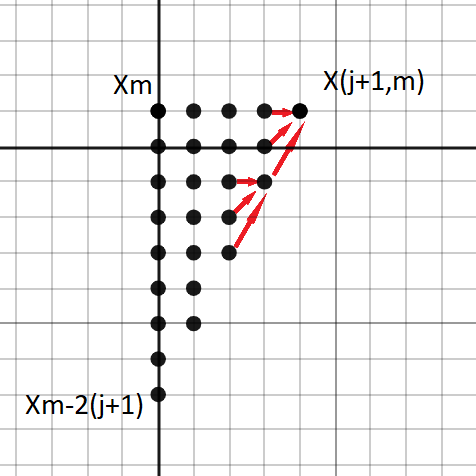
\includegraphics[width=2.5in]{CFLcondition.png}
  \end{center}
\end{figure}
\newpage
$u_{j+1,m}$ depends on the point to the left of it, the point left and down, and the point left and 2 down. I only included arrows for 2 points to clearly demonstrate the pattern. The mesh is not exactly this size all the time. It could be bigger or smaller depending on which $x_{j+1,m}$ time step we are interested in. \newline

From the graph we can see that:
\bea
 x_{m-2(j+1)} \leq \xi \leq  x_{m}
\eea

We know that the level curves of the solution, $\xi$, that give us accurate results as time moves forward need to pass through the point of interest $x_{j+1,m}$ and be inside the domain of dependence.\newline

This can be rewritten so we can solve for what the CFL condition is:  
\bea
 x_{m}-2(j+1)\Delta x \leq  x_{m}-c(j+1)\Delta t \leq  x_{m}+(j+1)\Delta t
\eea
We get from $x_{m}$ to $x_{m}-2(j+1)$ by (j+1) steps of whatever step size $\Delta x$ we choose. $\xi$ can be written in terms of how time is represented in the scheme - so t (from x - ct) changes to (j+1) steps of whatever step size $\Delta t$ we choose. \newline

Let's solve for the CFL condition:

Subtract $x_m$ from all sides:
\bea
-2(j+1)\Delta x \leq -c(j+1)\Delta t \leq (j+1)\Delta t
\eea

Divide by $(j + 1)\Delta x$:

\bea
-2 &\leq& -c\dfrac{\Delta t}{\Delta x}\ \leq 1 \\
\eea

c is still the wave speed constant and slope of the level curve. C can be anything, and to pass the CFL condition, we just need need to adjust $\Delta t$ and $\Delta x$ to make the value of $-c\dfrac{\Delta t}{\Delta x}$ in between -2 and 1.
\newline

In cases where c is a non-constant wave speed, the level curves become curves and not lines. To pass the CFL condition with non-constant wave speed, the characteristic curves passing through $x_{j+1,m}$ need to stay inside the domain of dependence the whole time they pass through those time steps. Therefore, these curves follow the same idea, that they are using only information relevant to the solution, as lines do because lines automatically stay inside the domain of dependence for all relevant time steps.

\subsection{Implementing an Explicit Difference Method}
% \red{Explain what an explicit difference method is. Explain what a boundary value problem is. Then present the sample problem from the text, with its solution, including reproductions of the graphs, and the sample problem you solved with me for mastery with its solution. Include your code here with clear explanations of what values must be changed to solve the two different problems. What follows is a sample MATLAB program that I wrote as an example of how to include commented code in a \LaTeX file.}
% \begin{verbatim}
% %% main_program.m
% %%    Find the first 5 normalized eigenfunctions for Schrodinger's equation 
% % %                   using the shooting method
% clear variables; close all; clc
% tol = 10^(-4);   % set the tolerance to work within
% col=['r','b','g','c','m','k','y']; % eigenfunction colors
% K = 1;                 % normalize to km/hbar^2 = 1
% epsn = .9;             % define the initial parameter epsilon_n
% psi=1;                 % define the initial guess for psi
% L = 4;                 % range to work in
% A = sqrt(L^2-epsn)*psi;   %left boundary differential
% x0 = [psi A];          % provide the initial conditions x1(-4) = 1, x1'(-4) = 2
% xp = -L:.1:L;          % define the span of the computational domain
% eigvalues = zeros(5,1);              % define the results matrices
% eigfunctions = zeros(length(xp),5);
% epsilon_start = epsn;    % beginning value of epsilon
% for modes = 1:5              % begin mode loop
%     epsilon = epsilon_start; % initial value of eigenvalue epsilon
%     deps = .05;              % default step size in epsilon
%     for j = 1:1000           % begin convergence loop for epsilon
%         x0 = [psi sqrt(L^2 - epsilon)*psi]; % Update initial condition for our new epsilon
%         [t,y] = ode45(@(t,y) schrodinger(t,y,K,epsilon), xp, x0); % solve ODEs
%         % Are we within tolerance?
%         if (abs(-sqrt(L^2-epsilon)*y(end,1)-y(end,2))<tol)
%             break                       % get out of convergence loop
%         end
%         % here we check to see if epsilon needs to be higher or lower
%         % then we bisect to get closer to our required tolerance
%         if (-1)^(modes)*(-sqrt(L^2-epsilon)*y(end,1)-y(end,2))>0     
%             epsilon = epsilon+deps;    
%         else
%             epsilon = epsilon - deps/2;
%             deps = deps/2;
%         end                             % end bisection loop
%     end                % end convergence loop
    
%     eigvalues(modes) = epsilon;
%     epsilon_start = epsilon+.1;    % after finding eigenvalue, pick
%                                     % new starting value for next higher
%                                     % mode
%     norm = trapz(t,y(:,1).*y(:,1));    % calculates the normalization
    
%     if modes > 0
%     plot(t,y(:,1)/sqrt(norm),col(modes)); hold on   % plot modes
%     end
    
%     eigfunctions(:,modes) = y(:,1)/sqrt(norm);
    
% end        % end modes loop
% \end{verbatim}

\subsection{Implementing an Implicit Difference Method}
%\blue{Explain what an implicit difference method is. Then present the sample problem from the text, with its solution and the sample problem you solved with me for mastery with its solution. Include your code here with clear explanations of what values must be changed to solve the two different problems.
%What follows is a sample using a block quotation and reference.}
%J. D. Lambert described the phenomenon of stiffness for a system of
%differential equations as follows:
%\begin{quote} If a numerical method with a finite region of absolute stability,
%    applied to a system with any initial conditions, is forced to use in a
%    certain interval of integration a steplength which is excessively small in
%    relation to the smoothness of the exact solution in that interval, then the
%    system is said to be stiff in that interval. \cite{wikistiff}
%    \end{quote}
    
    
\section{The Method of Characteristics}
%\red{Give an introduction to the method of characteristics.}
The method of characteristics is used to solve first order linear and non-linear PDEs of the form $u_t+cu_x = d$.
C can take the form of a constant or a polynomial and the equation could be homogeneous or non-homogeneous. The method of characteristics can be used to solve first order nonlinear PDEs as well, where c is a function of u. Using the method of characteristics requires an initial condition $u(0,x)=f(x)$ and that we consider what is happening with the level curves of our solution on the $t,x$ plane. We will see what happens when c is a constant, a polynomial, and non-linear. 

\subsection{Solving $u_t+cu_x +du = g(x)$ with $u(0,x)=f(x)$}
%\blue{Explain how to solve such a problem when $c$ and $d$ are constants. Then present your solution to the mastery problem I gave you.}

First, let's consider what we know about $u(t,x)$ and $u(0,x)=f(x)$. \\

The level curves of the solution u(t,x) on the $t,x$ plane are curves of constant value for u(t,x). No matter which point we choose on the curve, we get the same value for u(t,x). A characteristic variable $\xi$ can be introduced that we choose to define as $\xi = x-ct$. $\xi$ represents a level curve of the solution on the $t,x$ plane where $c$ is a constant slope and $\xi$ is the x-intercept.\\

Since we know the initial condition $u(0,x) = f(x)$, we know what the solution looks like at $t=0$. If every point on our level curve gives the same value for $u(t,x)$, we can go to where $t=0$ on our level curve, which is equal to $\xi$, and know the value of the function. $\xi$ will be exactly $f$ at time 0. Therefore, $f(\xi)$ = $f(x)$ and we can plug in $\xi$ for x in the initial condition to get $u(t,x)$ \\

The mastery problem I was given: Find $u(t,x)$ given $u_t-5u_x=12$ with $u(0,x) = \dfrac{\mbox{arctan($x$)}}{(x^2+1)}$ \\

First, solve the homogeneous case for u(t,x). That means to solve $u_t-5u_x=0$.\newline 

The level sets of the solution look like:
\bea
h = u(t,x(t)) = \mbox{constant} \\
\eea

Take the normal derivative of both sides.
\bea
\dfrac{dh}{dt} &=& 0  = \dfrac{du}{dt}\dfrac{dt}{dt} + \dfrac{dx}{dt}\dfrac{du}{dx}\\
\eea

This looks like the given equation when:
\bea
c &=& \dfrac{dx}{dt} = -5 \\
\xi &=& x-ct \\
\xi &=& x+5t  \\
u(t,x) &=& \dfrac{\mbox{arctan}(x+5t)}{((x+5t)^2+1)}  \\
\eea

Now, let's see what we can add on to $u(t,x)$ by considering the constant on the right side of the PDE.\\
\bea
\dfrac{dh}{dt} &=& 12 \\
h &=& 12t + g(\xi) \\ 
\eea

We know the form of $g(\xi)$. It is the homogeneous solution we just calculated above. 
\bea
u(t,x) &=& \dfrac{\arctan(x+5t)}{((x+5t)^2+1)} + 12t \\
\eea


\subsection{Solving the linear transport equation with polynomial coefficients}
%\red{Explain how to solve such a problem when the wave speed is polynomial in $t$ or polynomial in $x$. Then demonstrate the solution with the mastery problem I gave you to solve.}
%The function u depends on t and x but x depends on t, so we can say that: \\
%\bea
%u(t,x(t)) = v = constant value \\
%\eea
We can solve linear transport equations with polynomial coefficients using the same idea as when they had constant coefficients. However, because the wave speed $c$ is not a constant, we can't find $\xi$ right away and will need to solve for it with separation of variables and integration. \newline

The mastery problem I was given: Find $u(t,x)$ given $u_t+(x^2+1)\sin(t)u_x=0$ with $u(0,x) = e^{-x^2}\cos(x)$ \\

The level sets of the solution look like:
\bea
h(t) = u(t,x(t)) = \mbox{constant}\\
\eea

Take the normal derivative of both sides:
\bea
\dfrac{dh}{dt} &=& \dfrac{du}{dt}\dfrac{dt}{dt} + \dfrac{dx}{dt}\dfrac{du}{dx} = 0\\
\eea

This looks like the given equation when:
\bea
\dfrac{dx}{dt} &=& (x^2+1)\sin(t) \\
\eea

Separation of variables:
\bea
\dfrac{dx}{(x^2+1)} &=& \sin(t)dt \\
\eea

Integrate and solve for $\xi$:
\bea
\int_{\xi}^{x} \dfrac{1}{(x^2+1)}dx &=& \int_{0}^{t} \sin(t)dt\\
\arctan(x)\Big|_\xi^x &=& -\cos(t)\Big|_0^t\\
\tan^{-1}(x)-\tan^{-1}(\xi) &=& -\cos(t) + 1\\
\tan^{-1}(\xi) &=& \tan^{-1}(x) + \cos(t) - 1\\
\xi &=& \tan(\tan^{-1}(x) + \cos(t) - 1)\\
\eea 


Plug back in to the initial condition $u(0,x) = e^{-x^2}\cos(x)$:
\bea
u(t,x) = e^{-(\tan(\tan^{-1}(x) + \cos(t) - 1))^2}\cos(\tan(\tan^{-1}(x) + \cos(t) - 1))\newline
\eea
In this case, there is nothing more to add on at the end because the given function was homogeneous.




\subsection{Solving first order nonlinear PDEs using the method of characteristics}

%\blue{Explain how to solve a problem of the form $u_t+g(u)u_x=0$. Then solve the mastery problem I gave you to solve. What follows is a sample use of equation array and piecewise defined functions.}
% \bea
%y_{n+1} &=& y_n+\red{e} + \Delta t \lambda y_{n+1} \\
%\left(1-\Delta t
%\lambda\right)^ny_{n+1} &=& y_n+\red{e} \\
%y_{n+1} &=& \left(\frac{1}{1-\Delta t \lambda}\right)(y_n+\red{e}) \\
%y_{n+1} &=& \left(\frac{1}{1-\Delta t \lambda}\right)^{n+1}(y_0+\red{e}) 
%\eea
%and hence a global error after $N$ steps of
%$$E = \left(\frac{1}{1-\Delta t \lambda}\right)^N\red{e}.$$ Therefore
%$$\lim_{N\to \infty} E = \begin{cases} \infty & 
%  |1-\Delta t \lambda|<1 \\
% 0 &  |1-\Delta t \lambda|>1 \\
%  \red{e} & |1-\Delta t \lambda|=1
%  \end{cases}.$$


\subsection{Shocks}
%\red{Explain how to recognize and solve a first order differential equation whose solution will involve a shock. Then solve the mastery problem I gave you. What follows is sample code for including a figure, Figure~\ref{fig:example}, with a caption and label.}
%\begin{figure}[ht]
%\begin{center}
%  \includegraphics[width=2.5in]{stability-backwardeuler}
%  \end{center}
%\caption{Stable regions for forward (left) and backward (right) Euler methods %where green is
%  convergent and white is divergent. \label{fig:example}}
%\end{figure}
\subsection{Rarefaction Waves}
%\blue{Explain how to recognize and solve a first order differential equation that will result in a rarefaction wave. Then solve the mastery problem I gave you. What follows is sample code for a table. I have left some horizontal and vertical lines out for demonstration purposes, and doubled others.}
%\begin{center}
%\begin{tabular}{|l|ccc|} \hline
%\textbf{Command} & \textbf{Local Error} & \textbf{Global Error} & %\textbf{Scheme} \\ \hline \hline  
%  \texttt{ode23} & $O(\Delta t^3)$ & $O(\Delta t^2)$ & Runge-Kutta\\
%  \texttt{ode45} & $O(\Delta t^5)$ & $O(\Delta t^4)$ & Runge-Kutta \\ \hline
%  \texttt{ode15s} & variable  & variable & Gear's method, stiff\\
%  \texttt{ode113} & variable & variable & predictor/corrector \\ \hline
%  \end{tabular}
%  \end{center}
%For more information, see the Matlab documentation \cite{matlabode}.

\section{Fourier Series}
%\blue{Give an introduction to Fourier series.}
Fourier series approximate functions with an infinite series of sines and cosines. They can be used to approximate real functions and complex functions. A complex Fourier Series can be written in terms of exponentials or sines and cosines because of their relationship for complex functions but will still be an infinite series. \newline
A Fourier Series will only match the function it's approximating on the interval its Fourier Coefficients were integrated on because Fourier Series are periodic on intervals of $2L$, where $-L$ to $L$ is the interval the function is being approximated on. 

\subsection{Real Fourier Series}
%\red{Explain how to calculate the real Fourier series for a suitable function. Then present the example that you solved for your mastery check.}
A real Fourier Series has the form:
\bea
f(x) &\approx& \dfrac{a_0}{2}+\sum_{k=1}^{\infty} a_k\cos(kx)+b_k\sin(kx) \\
\eea
Where $a_k$ and $b_k$ are the $L_2$ inner product of the function $f(x)$ and $\cos(kx)$ and $\sin(kx)$: 
\bea
a_k &=& <f(x),\cos(kx)> = \dfrac{1}{\pi}\int_{-\pi}^{\pi} f(x)\cos(kx)dx, \hspace{.2in} k\geq0 \hspace{.1in} integers \\
b_k &=& <f(x),\sin(kx)> = \dfrac{1}{\pi}\int_{-\pi}^{\pi} f(x)\sin(kx)dx, \hspace{.2in} k\geq1 \hspace{.1in} integers \\
\eea
We can extend a Fourier Series to an interval $-L$ to $L$ with the form:
\bea
f(x) &\approx& \dfrac{a_0}{2}+\sum_{k=1}^{\infty} a_k\cos\left(\dfrac{k \pi x}{L}\right)+b_k\sin\left(\dfrac{k \pi x}{L}\right) \\
\eea
where:
\bea
a_k &=& <f(x),\cos(kx)> = \dfrac{1}{L}\int_{-L}^{L} f(x)\cos\left(\dfrac{k \pi x}{L}\right)dx, \hspace{.2in}  k\geq0 \hspace{.1in} integers \\
b_k &=& <f(x),\sin(kx)> = \dfrac{1}{L}\int_{-L}^{L} f(x)\sin\left(\dfrac{k \pi x}{L}\right)dx, \hspace{.2in} k\geq1 \hspace{.1in} integers \\
\eea
The mastery problem I was given:\newline

Find the Fourier Series for $f(x)=|x|$ on [-3,3]\newline

Since we are on $[-L,L]$, the Fourier Series will have the form:
\bea
f(x) &\approx& \dfrac{a_0}{2}+\sum_{k=1}^{\infty} a_k\cos\left(\dfrac{k \pi x}{L}\right)+b_k\sin\left(\dfrac{k \pi x}{L}\right) \\
\eea

Solve for $a_k$:
\bea
a_k &=& \dfrac{1}{3}\int_{-3}^{3} |x|\cos\left(\dfrac{k \pi x}{3}\right)dx\\
a_k &=& \dfrac{6(\pi k \sin(\pi k)+\cos(\pi k) -1)}{\pi^2 k^2}\\
\eea

$a_k$ can be simplified to the following because $sin(\pi k)$ is always 0 and $cos(\pi k)$ is $(-1)^k$:
\bea
a_k &=& \dfrac{6((-1)^k-1)}{\pi^2 k^2}\\
\eea

Solve for $b_k$:
\bea
b_k &=& \dfrac{1}{3}\int_{-3}^{3} |x|\sin\left(\dfrac{k \pi x}{3}\right)dx\\
b_k &=& 0
\eea

$b_k$ = 0 because the inner product of an even and an odd function is always 0.\newline 

Now that we have $a_k$ and $b_k$ did we make any assumptions that are easy to overlook?\newline

When solving for $a_k$ we assumed that k was not equal to 0. If k = 0 then we are left with:
\bea
a_0 &=& \dfrac{1}{3}\int_{-3}^{3} |x|dx\\
a_0 &=& 3
\eea

The Fourier Series for $f(x) = |x|$ on [-3,3] has the form:
\bea
f(x) &\approx& \dfrac{3}{2}+\sum_{k=1}^{\infty} \dfrac{6((-1)^k-1)}{\pi^2 k^2}\cos\left(\dfrac{k \pi x}{3}\right) \\
\eea

\subsection{Complex Fourier Series}
%\blue{Explain how to calculate the complex Fourier series for a suitable function. Then present the example that you solved for your mastery check.}
A Complex Fourier Series has the form:
\bea
f(x) &\approx& \sum_{k=1}^{\infty} c_ke^{ikx} \\
\eea
where $c_k$ is the Hermitian inner product of $f(x)$ and $e^{ikx}$. This means we need the conjugate of $e^{ikx}$ when doing the integral for the inner product.
\bea
c_k &=& <f(x),e^{ikx}> = \dfrac{1}{2\pi}\int_{-\pi}^{\pi} f(x)e^{-ikx}dx \\
\eea
The mastery problem I was given: \newline

Find the Complex Fourier Series for $f(x) = sin^3(x)+cos^2(5x)$ on $[-\pi,\pi]$

Solve for $c_k$:
\bea
c_k &=& \dfrac{1}{2\pi}\int_{-\pi}^{\pi} (sin^3(x)+cos^2(5x))e^{-ikx}dx\\
c_k &=& \left(\dfrac{1}{2\pi}\right)\left(\dfrac{2(k^6-60k^4-6ik^3+509k^2+600ik-450)\sin(\pi k)}{k(k^6-110k^4+1009k^2-900)}\right)\\
\eea

$c_k$ will equal 0 for all k's except when the denominator is equal to 0. This is because $sin(\pi k)$ is always equal to 0.\\

If we solve for k when the denominator is equal to 0, we can find the values for $c_k$ that need to be computed separately. \newline

$k(k^6-110k^4+1009k^2-900)=0$ when k = -10, -3, -1, 0, 1 \\

Solve for $c_k$ when k = -10,-3,-1,0,1 - don't forget to divide by $2\pi$ for each integral:\newline

\bea
c_{-10} &=& \dfrac{1}{4} \\
c_{-3} &=& \dfrac{-i}{8} \\
c_{-1} &=& \dfrac{3i}{8} \\
c_0 &=& \pi \\
c_1 &=& \dfrac{-3i}{8}\\
\eea

The complex Fourier Series for $f(x) = sin^3(x)+cos^2(5x)$ on $[-\pi,\pi]$ looks like:
\bea
f(x) &\approx& \sum_{k=1}^{\infty} c_{-10}e^{ikx} + c_{-3}e^{ikx} + c_{-1}e^{ikx} + c_{0}e^{ikx} + c_{1}e^{ikx} \\
f(x) &\approx& \sum_{k=1}^{\infty} \dfrac{1}{4}e^{ikx} + \dfrac{-i}{8}e^{ikx} + \dfrac{3i}{8}e^{ikx} + \pi e^{ikx} + \dfrac{-3i}{8}e^{ikx} \\
f(x) &\approx&  \sum_{k=1}^{\infty} \dfrac{1}{4}e^{ikx} + \dfrac{-i}{8}e^{ikx} + \pi e^{ikx}\\
\eea



\subsection{Convergence of Fourier Series}
%\red{Discuss the convergence of Fourier series. Then present the example that you solved for your mastery check.}

\subsection{Integrability and Differentiability of Fourier Series}
%\blue{Discuss the integrability and differentiability of Fourier series. Then present the example that you solved for your mastery check.}

\subsection{Boundary Conditions}
%\red{Discuss the various standard types of boundary conditions and what conditions tell you about the form of a Fourier Series solution. Then present the example that you solved for your mastery check.}

\section{Separation of Variables}
%\red{Give an overview of the method of separation of variables.}
Separation of Variables assumes the solution to a PDE can take the form of the product of two functions w(t) and v(x). Therefore, u(t,x) = w(t)v(x). We will use separation of variables to solve heat equations, wave equations, and Laplace equations and see what the solutions for w(t), v(x), and u(t,x) look like in each case. We can also use this idea to see what the equilibrium solution for a u(t,x) looks like. 
\subsection{Equilibrium behavior of a solution}
%\red{Explain what equilibrium behavior is and how one goes about finding the equilibrium behavior of a system. Then give the example that you solved for your mastery check.}

Equilibrium behavior for a solution u(t,x) is what is happening with the solution at $t=\infty$. Equilibrium solutions are independent of t at the end so we will only have a function of x. \newline
The Mastery problem I was given: 

Find the equilibrium solution for the heat equation $u_t &=& .005 u_{xx}$ given the following initial and boundary conditions:
\bea
u(0,x) &=& f(x) \\
u(t,0) &=& 6 \\
u(t,5) &=& -3 \\
\eea
Note: An equilibrium solution for a heat equation would be a temperature. For it to be an equilibrium solution, the behavior would have to approach an actual value.\newline

If an equilibrium solution exists, it will take the form:
\bea
u^{\star}(x) = \lim_{t\to\infty} u(t,x) 
\eea

Since our heat equation has both $u_t$ and $u_{xx}$, lets find the PDE that  $u^{\star}(x)$ satisfies:
\bea
\frac{\partial u^{\star} }{\partial t} &=& 0 \\
\eea

because $u^{\star}$ doesn't depend on t at all, and 
\bea
\frac{\partial u^{\star} }{\partial x} &=& (u^{\star})'' \\
\eea

because $u^{\star}(x)$ is a function of $x$.\\

Plug in to heat equation to get the form of it:
\bea
0 &=& .005(u^{\star})''
\eea

This tells us that $u^{\star}(x)$ looks like:
\bea
u^{\star}(x) = Ax + B
\eea

$u^{\star}(x)$ looks like this because we want the second derivative of $u^{\star}$ to equal 0 so $u^{\star}(x)$ needs to have this form. 

We can find A and B using initial conditions:

We know that:
\bea
u^{\star}(0) &=& 6 \\
u^{\star}(5) &=& -3 \\
\eea

Solve for A and B:
\bea
A(0) + B &=& 6\\
B &=& 6 \\
A(5) + 6 &=& -3 \\
A &=& -\dfrac{9}{5} \\
\eea

The equilibrium solution for the given heat equation looks like:
\bea
u^{\star}(x)=-\dfrac{9}{5}(x) + 6
\eea

Note: If we the equilibrium solution to give us an actual value for a certain x, it limits what the 2nd order diff eq's can be to only ones where $u^{\star}$ works out nicely. The equilibrium solution could be a cycle or something but we are not interested in when that would be the case. 

\subsection{Solving the 1D heat equation}
%\blue{Explain how to solve the 1D heat equation with boundary conditions using the method of separation of variables. Then present the example that you solved for your mastery check.}
The heat equation is $u_t = \gamma u_{xx}$

Assume the solution looks like $u(t,x) = w(t)v(x)$

We found that:
\bea
\dfrac{\partial u}{\partial t} &=& w'(t)v(x) \\
\dfrac{\partial^2 u}{\partial x^2} &=& \gamma w(t)v''(x) \\
w'(t)v(x) &=& \gamma w(t)v''(x) \\
\dfrac{w'(t)}{w(t)} &=& \gamma \dfrac{v''(x)}{v(x)} = \mbox{constant} = -\lambda
\eea

This is constant because the only thing that can be both a function of t a function of x is a constant. We don't have to call it -$\lambda$, it could have been $\lambda$ if we wanted but it would change the way that the different cases for $\lambda$ look. \newline

We now have a system or first order normal differential equations that we can use to find the solution.
\bea
w'(t) &=& -\lambda w(t) \\
v''(x) &=& \dfrac{-\lambda}{\gamma}v(x) \\
\eea

We know that $u(t,x) = w(t)v(x)$ so we are interested in cases where both $w(t)$ and $v(x)$ are not equal 0 because if either $w(t)=0$ or $v(x)=0$, then we get the trivial solution $u(t,x) = 0$.\\

The mastery problem I was given: \newline

Find $u(t,x)$ for $u_t=.3u_{xx}$ given the following intial and boundary conditions:
\bea
u(0,x)&=&x^2-8x\\
u_x(t,0)&=&0\\
u_x(t,4)&=&0\\
\eea
Note: $\gamma=.3$ - that's gamma \newline
Note: This problem has Neumann (not Dirichlet) boundary conditions because they prescribe the derivative (not the function value) at the boundary. When doing the 3 cases for $\lambda$ we need to solve $v'(0)=0$ and $v'(0)=4$ not $v(0)=0$ and $v(0)=4$.\newline

We know the solutions for $w(t)=Ce^{-\lambda t}$. \\

We know the solutions for $v(x)$ will fall into 3 cases depending on if $\lambda > 0$, $\lambda < 0$, or $\lambda = 0$. \newline
Case 1: $\lambda$ = 0 
\bea
v(x) &=& Ax+B\\
v'(x) &=& A\\
\eea

Use the 1st boundary condition:
\bea
v'(0) &=& 0 = A\\
A &=& 0
\eea

Use the 2nd boundary condition:
\bea
v'(4) &=& 0 = A\\
A &=& 0
\eea

Tells us that A = 0 and B is unconstrained.\newline
Case 2: $\lambda > 0$ This will mean $\omega=\sqrt{\dfrac{\lambda}{\gamma}}$
\bea
v(x) &=& A\cos(\omega x)+B\sin(\omega x) \\
v'(x) &=& -A\omega \sin(\omega x)+B\omega \cos(\omega x)  \\
\eea

Use the 1st boundary condition:
\bea
v'(0) &=& 0 = B\omega\\
B &=& 0
\eea

Use the 2nd boundary condition: B = 0 so it's not in $v'(x)$ anymore.
\bea
v'(4) &=& 0 = -A\sin(\omega 4)\\
\eea

$-A\sin(\omega 4)$ equals 0 when $\omega = \dfrac{k\pi}{4}$. \newline
Case 3: $\lambda < 0$ This will mean $\omega=\sqrt{\dfrac{-\lambda}{\gamma}}$
\bea
v(x) &=& A\cosh(\omega x)+B\sinh(\omega x) \\
v'(x) &=& B\omega \cosh(\omega x)+A\omega \sinh(\omega x)  \\
\eea

Use the 1st boundary condition: \newline
Note: sinh(0) = 0 and cosh(0) = 1
\bea
v'(0) &=& 0 = B\omega\\
B &=& 0
\eea

Use the 2nd boundary condition: B = 0 so it's not in $v'(x)$ anymore.
\bea
v'(4) &=& 0 = -A\sinh(\omega 4)\\
\eea

Either:
\bea
A &=& 0 \\
or\\
\omega &=& 0 \\
or\\
\sinh(\omega 4) &=& 0
\eea

We know $\omega$ is positive so it can't equal 0.\newline 

$\sinh(\omega 4)$ equals 0 when evaluated at 0. However, we know that $\omega$ is positive so this can't happen. \newline

So A = 0 which makes this case trivial because both A = 0 and B = 0. \newline 

Put everything back together:

$v(x) = B$ with $\lambda=0$\newline 

$v(x) = A\cos\left(\frac{k \pi x}{L}\right)$ with $\lambda > 0$.  This is because we found that B = 0 when we solved and that $v(x)$ still equals $A\cos(\omega x)+B\sin(\omega x)$.  \newline

We have just found a whole set of solutions for $v(x)$: $v_0(x) = B$ and $v_k(x) = A_k\cos\left(\frac{k\pi x}{L}\right)$\\

w(t)=$Ce^{-\lambda t}$:

w(t) = constant with  $\lambda = 0$

w(t) =$Ce^{\dfrac{-k^2 \pi^2 \gamma }{L^2}t}$ with $\lambda > 0$

Note: \bea
\omega= \dfrac{k \pi}{L} &=& \sqrt{\dfrac{\lambda}{\gamma}} \\
\lambda &=& \dfrac{k^2 \pi^2 \gamma }{L^2} \\
\eea

$u(t,x) = w(t)v(x)$

$u(t,x) = a_0 + \sum_{k=1}^{\infty} a_k e^{\dfrac{-k^2 \pi^2 \gamma }{L^2}t} \cos\left(\frac{k \pi x}{4}\right)$ \\ 

I replaced B with $a_0$ and the C*A inside the sum with $a_k$ to make it look more like a Fourier Series. \\

We can still use $u(0,x)=x^2-8x$ as piece of information we haven't used.\\

$u(0,x)=x^2-8x$ = $a_0 + \sum_{k=1}^{\infty} a_k \cos\left(\frac{k \pi x}{4}\right)$ \\

This looks like a Fourier Cosine Series for f(x) on [0,4]. We want a Cosine Series on [-L,L]. We can use an even extension (because cosine is an even function) to get $a_0$ and $a_k$:

\bea
a_0 &=& \dfrac{1}{L}\int_{0}^{L} f(x)dx \\
a_k &=& \dfrac{2}{L}\int_{0}^{L} f(x)\cos\left(\frac{k \pi x}{L}\right)dx \\
\mbox{where}: \\
L&=&4\\
f(x) &=& x^2-8x
\eea

$a_0$ = $-\dfrac{32}{3}$

$a_k = -\dfrac{32((\pi^2 k^2 +2)sin(k \pi) - 2 \pi k)}{\pi^3 k ^3}$

$a_k = \dfrac{64 \pi k}{\pi^3 k ^3}$ because $sin(k\pi) = 0$ \newline

$a_k = \dfrac{64}{\pi^2 k ^2}$ \newline

$u(t,x) = -\dfrac{32}{3} + \sum_{k=1}^{\infty} \left(\dfrac{64}{\pi^2 k ^2}\right) e^{\dfrac{-k^2 \pi^2 .3 }{4^2}t} \cos\left(\dfrac{k \pi x}{4}\right)$ \\ 


\subsection{Solving the Laplace equation}
%\red{Explain how to solve the Laplace equation with boundary conditions using the method of separation of variables. Then present the example that you solved for your mastery check.}
 


\subsection{Solving the 1D wave equation}
%\red{Explain how to solve the 1D wave equation with boundary conditions using the method of separation of variables. Then present the example that you solved for your mastery check.}

\subsection{Solving the 1D wave equation using d'Alembert's formula}
%\red{Explain how to solve the 1D wave equation with boundary conditions using d'Alembert's formula. Then present the example that you solved for your mastery check.}
%\section{Bibliography}
\begin{bibdiv}
\begin{biblist}
\bibselect{numerical}
\end{biblist}
\end{bibdiv}
\end{document}